\providecommand\myClassOptions{}
\documentclass[a4paper,\myClassOptions]{article}
\usepackage{ngerman, textcomp}
\usepackage{pdfpages}

\begin{document}
\Large

Pagetemplate=1 (A4) \textrightarrow A4L und A3L werden skaliert
   A5 bleibt unveraendert.
\begin{verbatim}
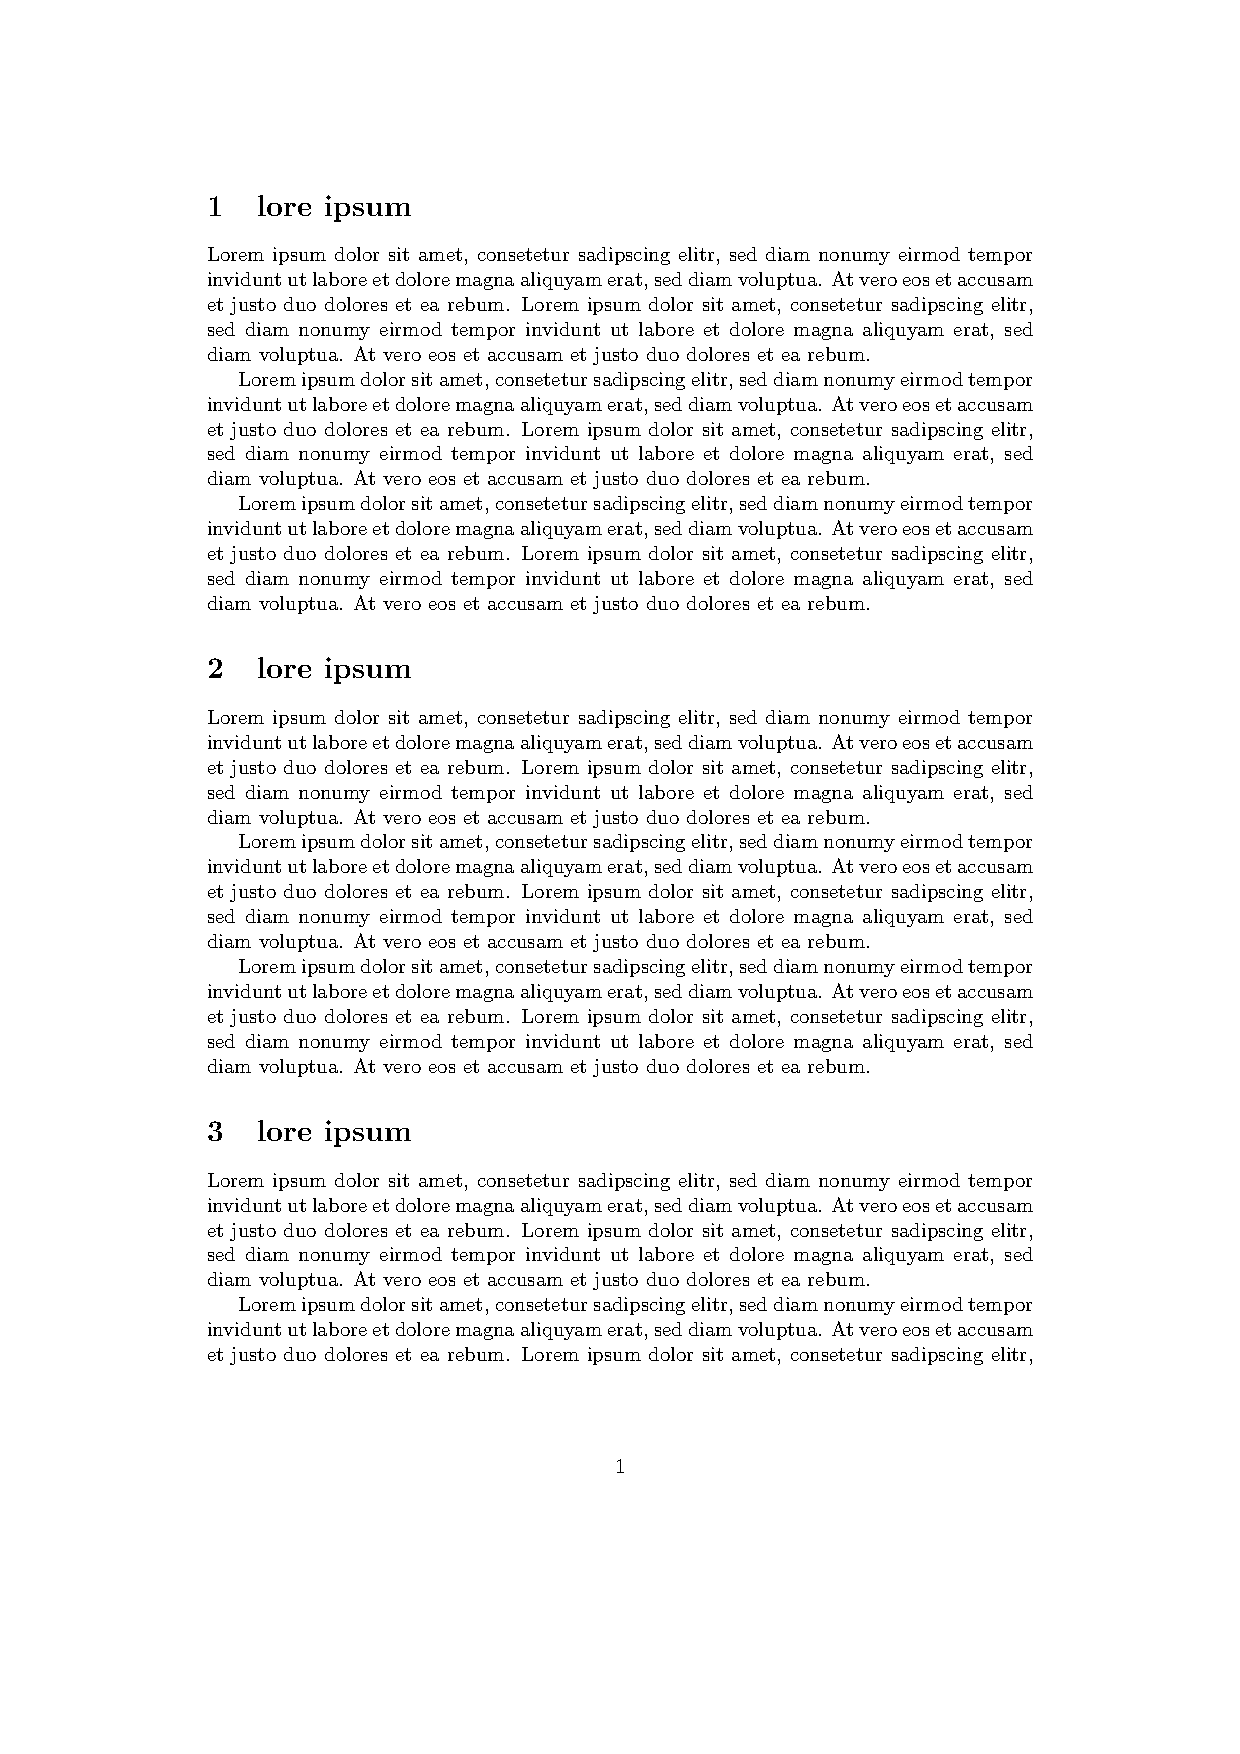
\includepdf[pages=-, nup=3x3,
            frame]{pdf/mix1.pdf}
\end{verbatim}
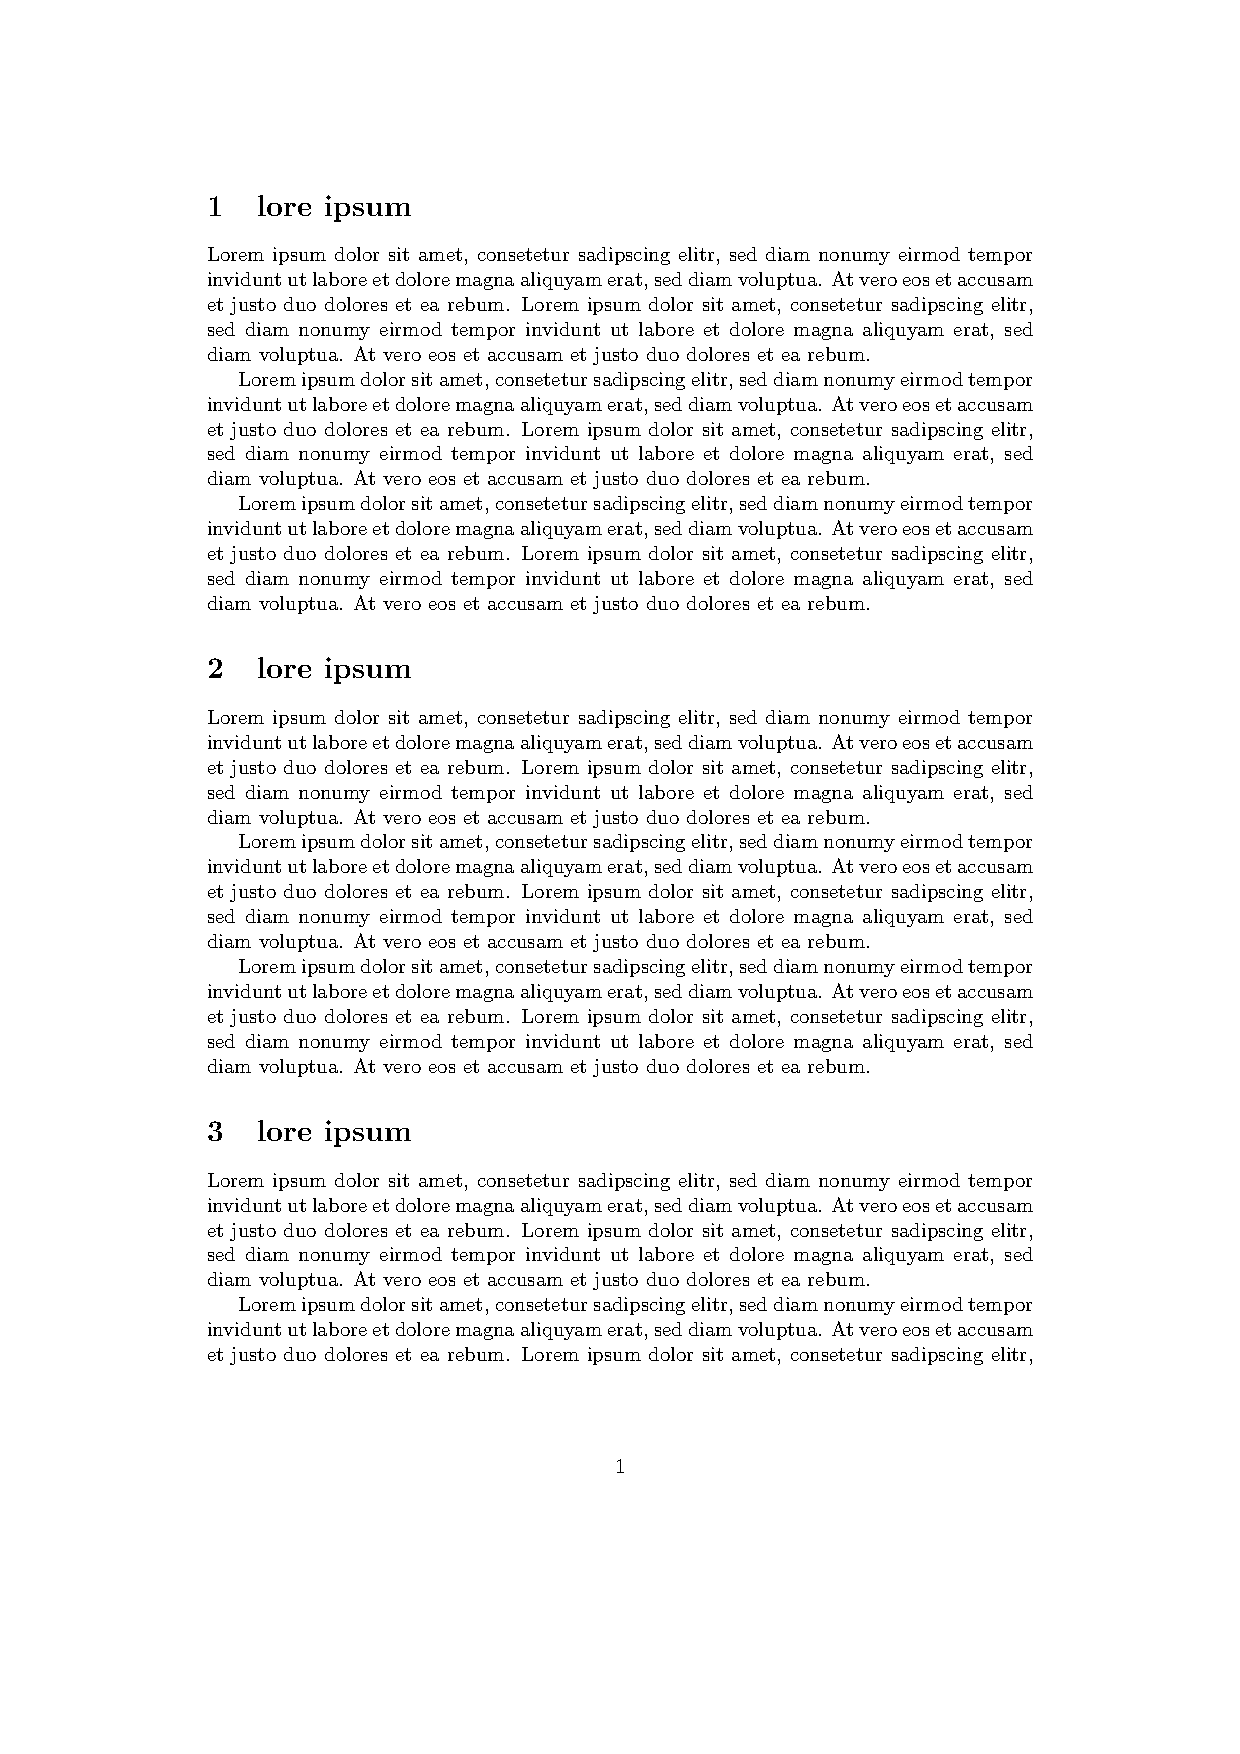
\includepdf[pages=-, nup=3x3,
            frame]{pdf/mix1.pdf}

Mit rotateoversize:
\begin{verbatim}
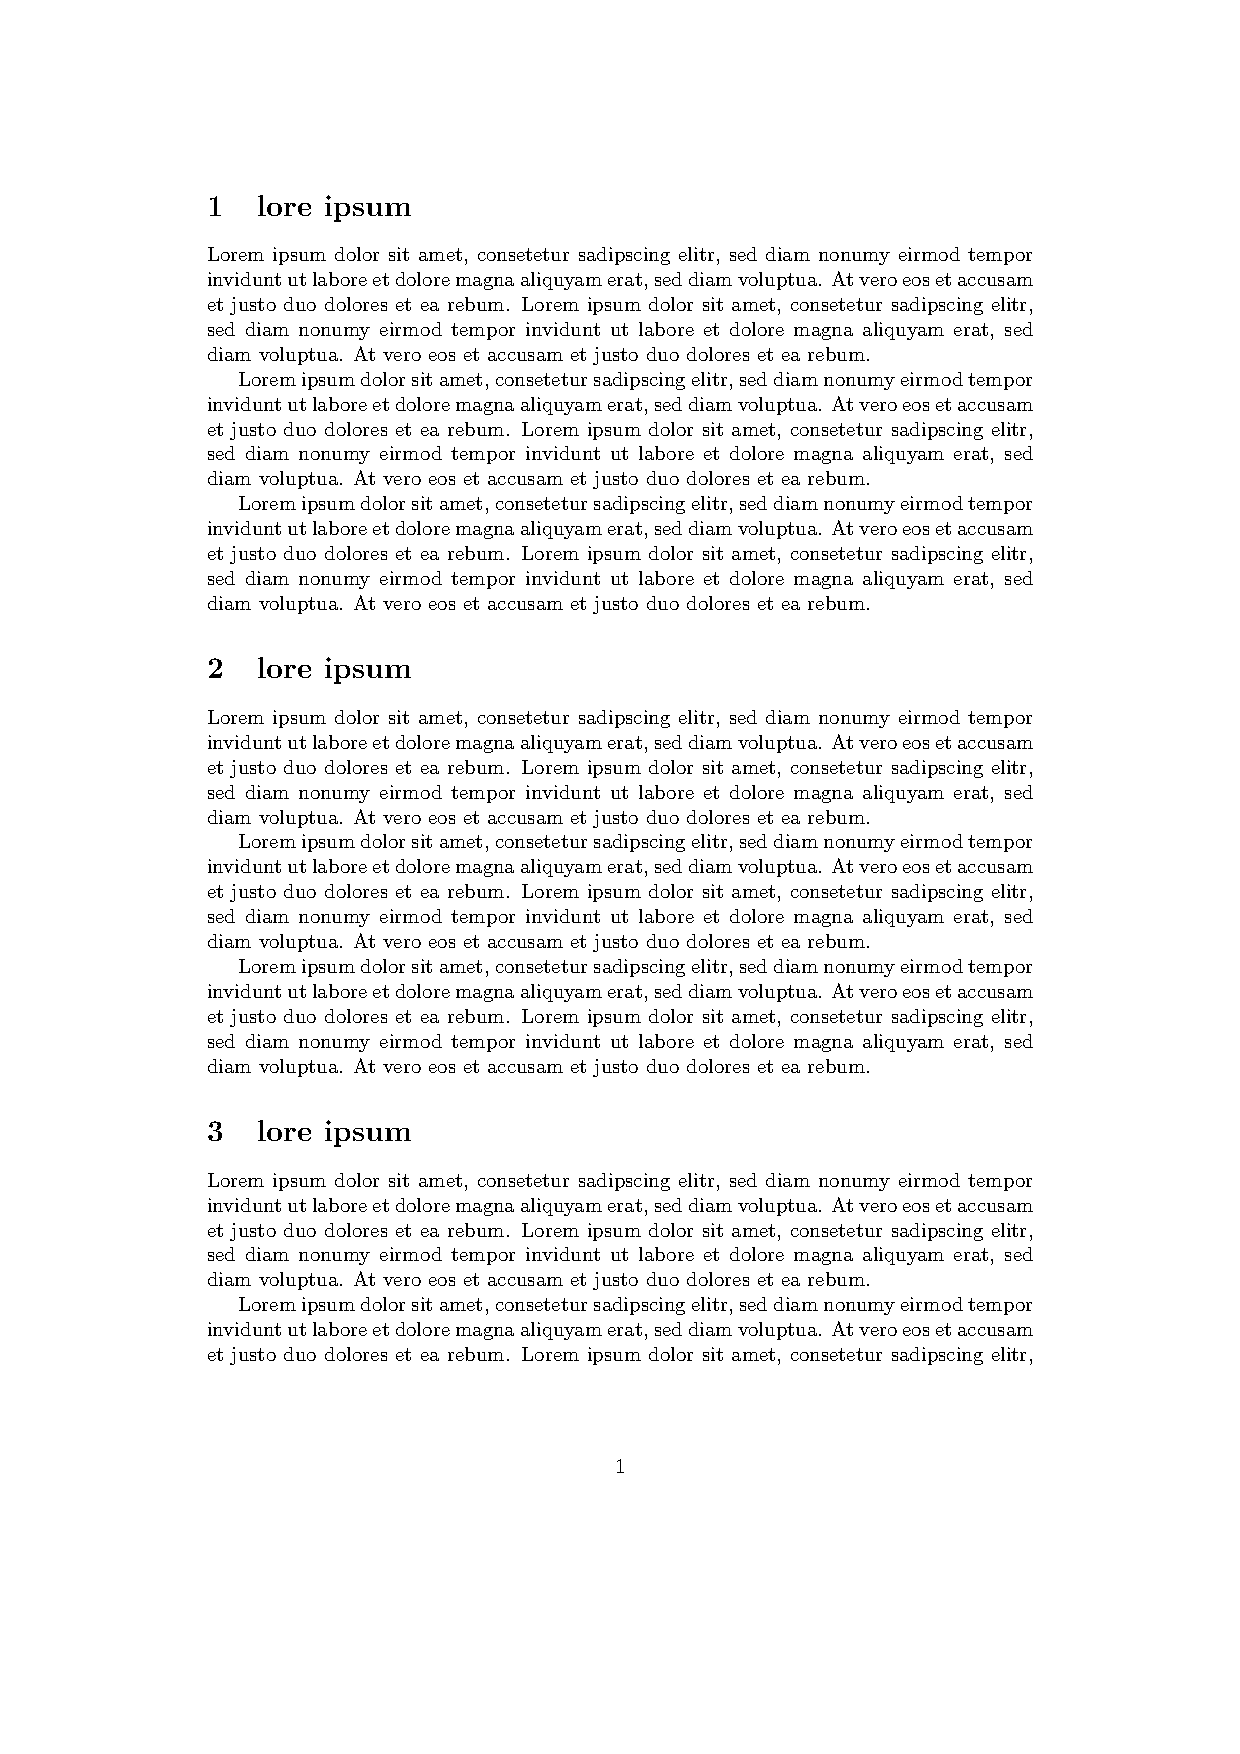
\includepdf[rotateoversize, pages=-, nup=3x3,
            frame]{pdf/mix1.pdf}
\end{verbatim}
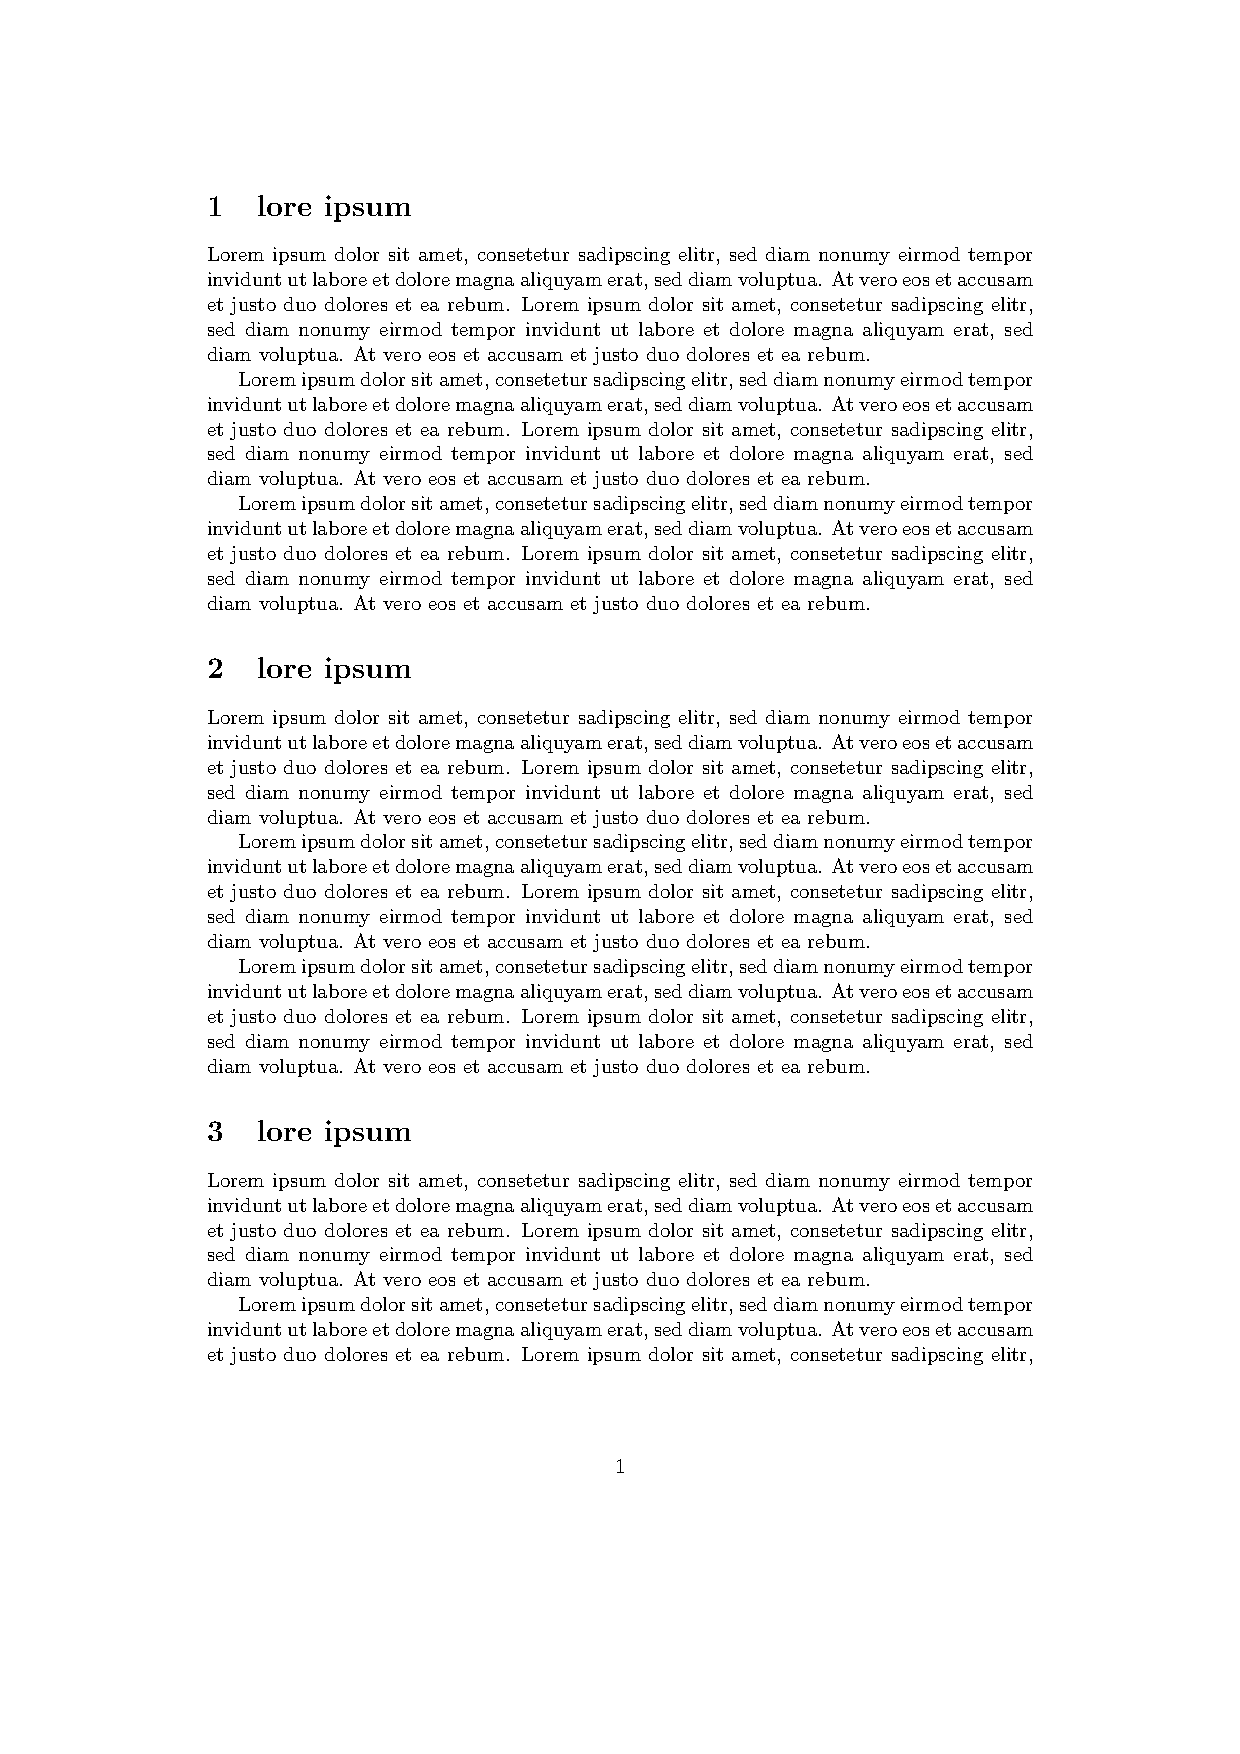
\includepdf[rotateoversize, pages=-, nup=3x3,
            frame]{pdf/mix1.pdf}

Pagetemplate=7 (A5) \textrightarrow A4P, A4L und A3L werden verkleinert.
\begin{verbatim}
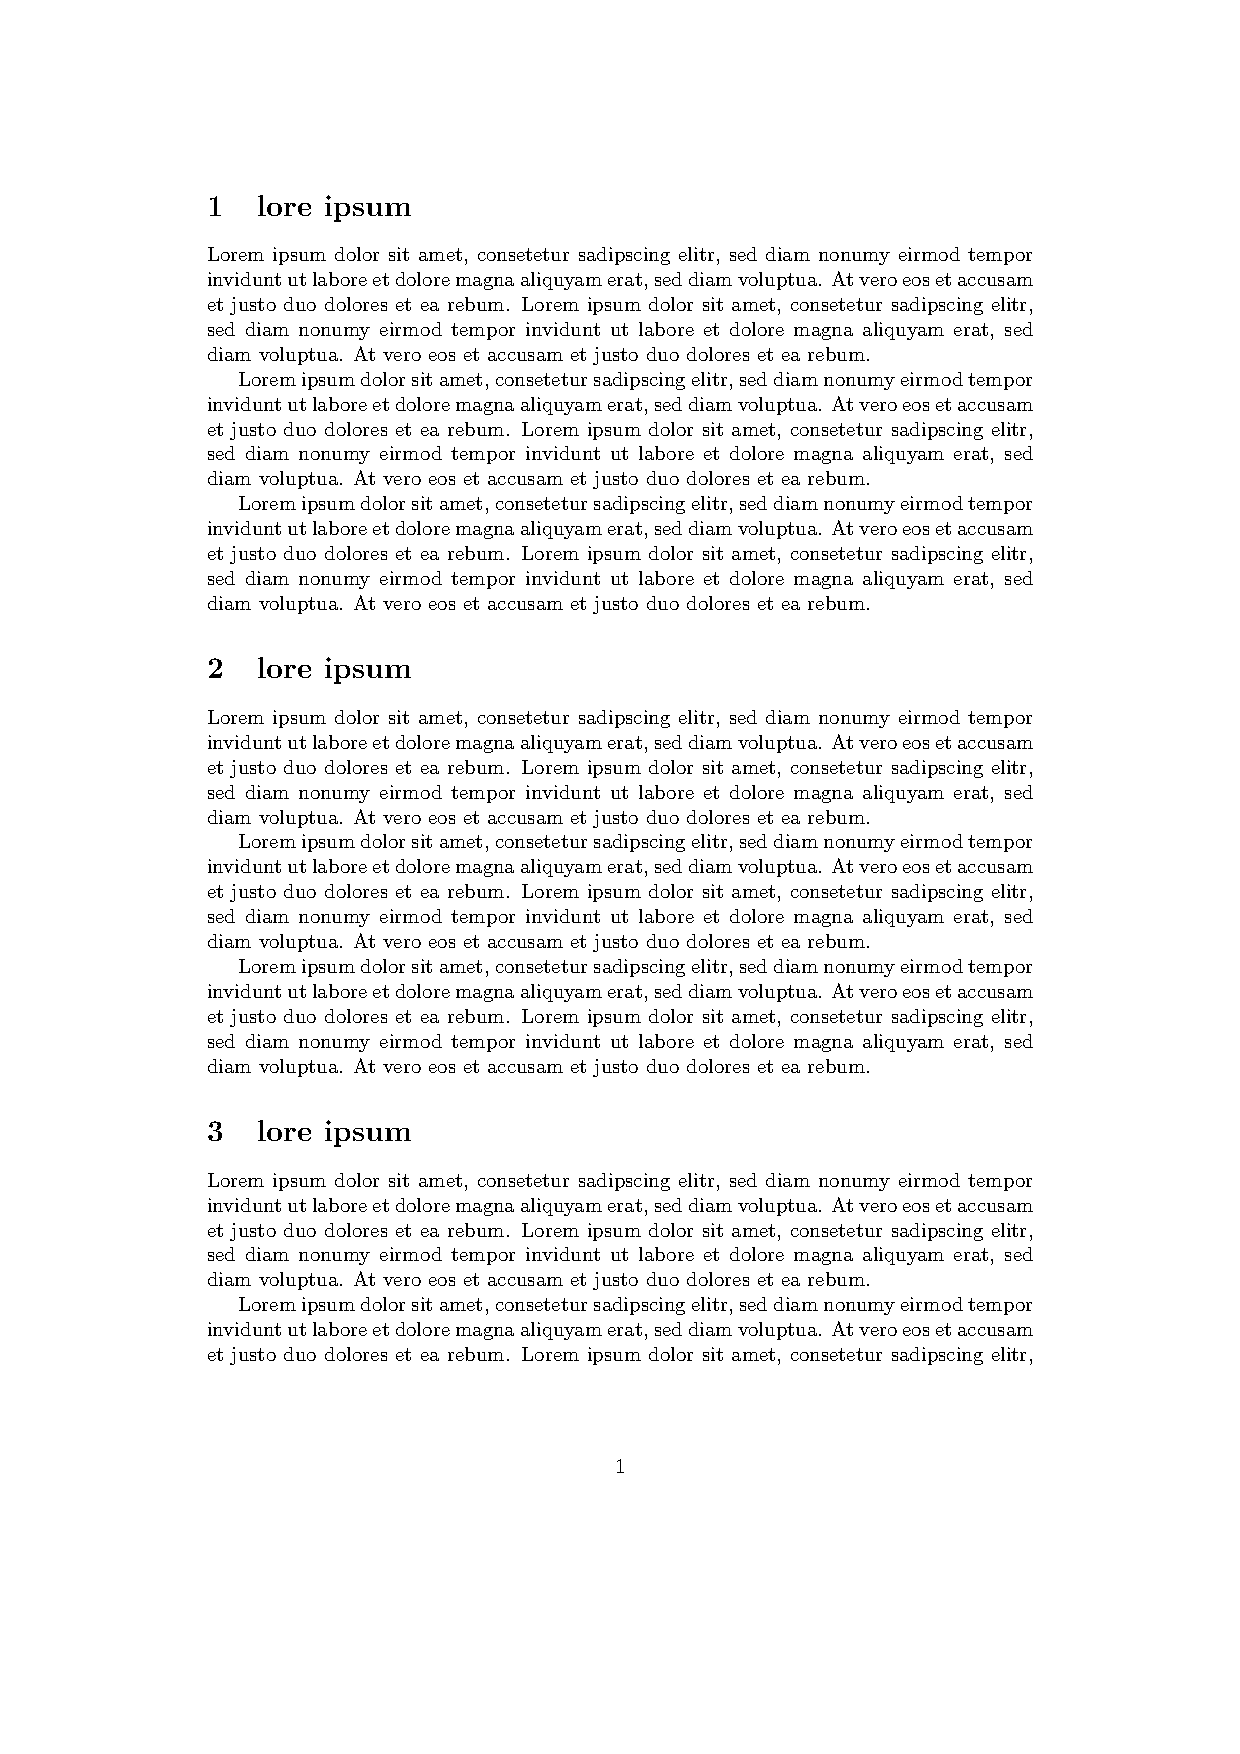
\includepdf[pagetemplate=7, pages=-, nup=3x3,
            frame]{pdf/mix1.pdf}
\end{verbatim}
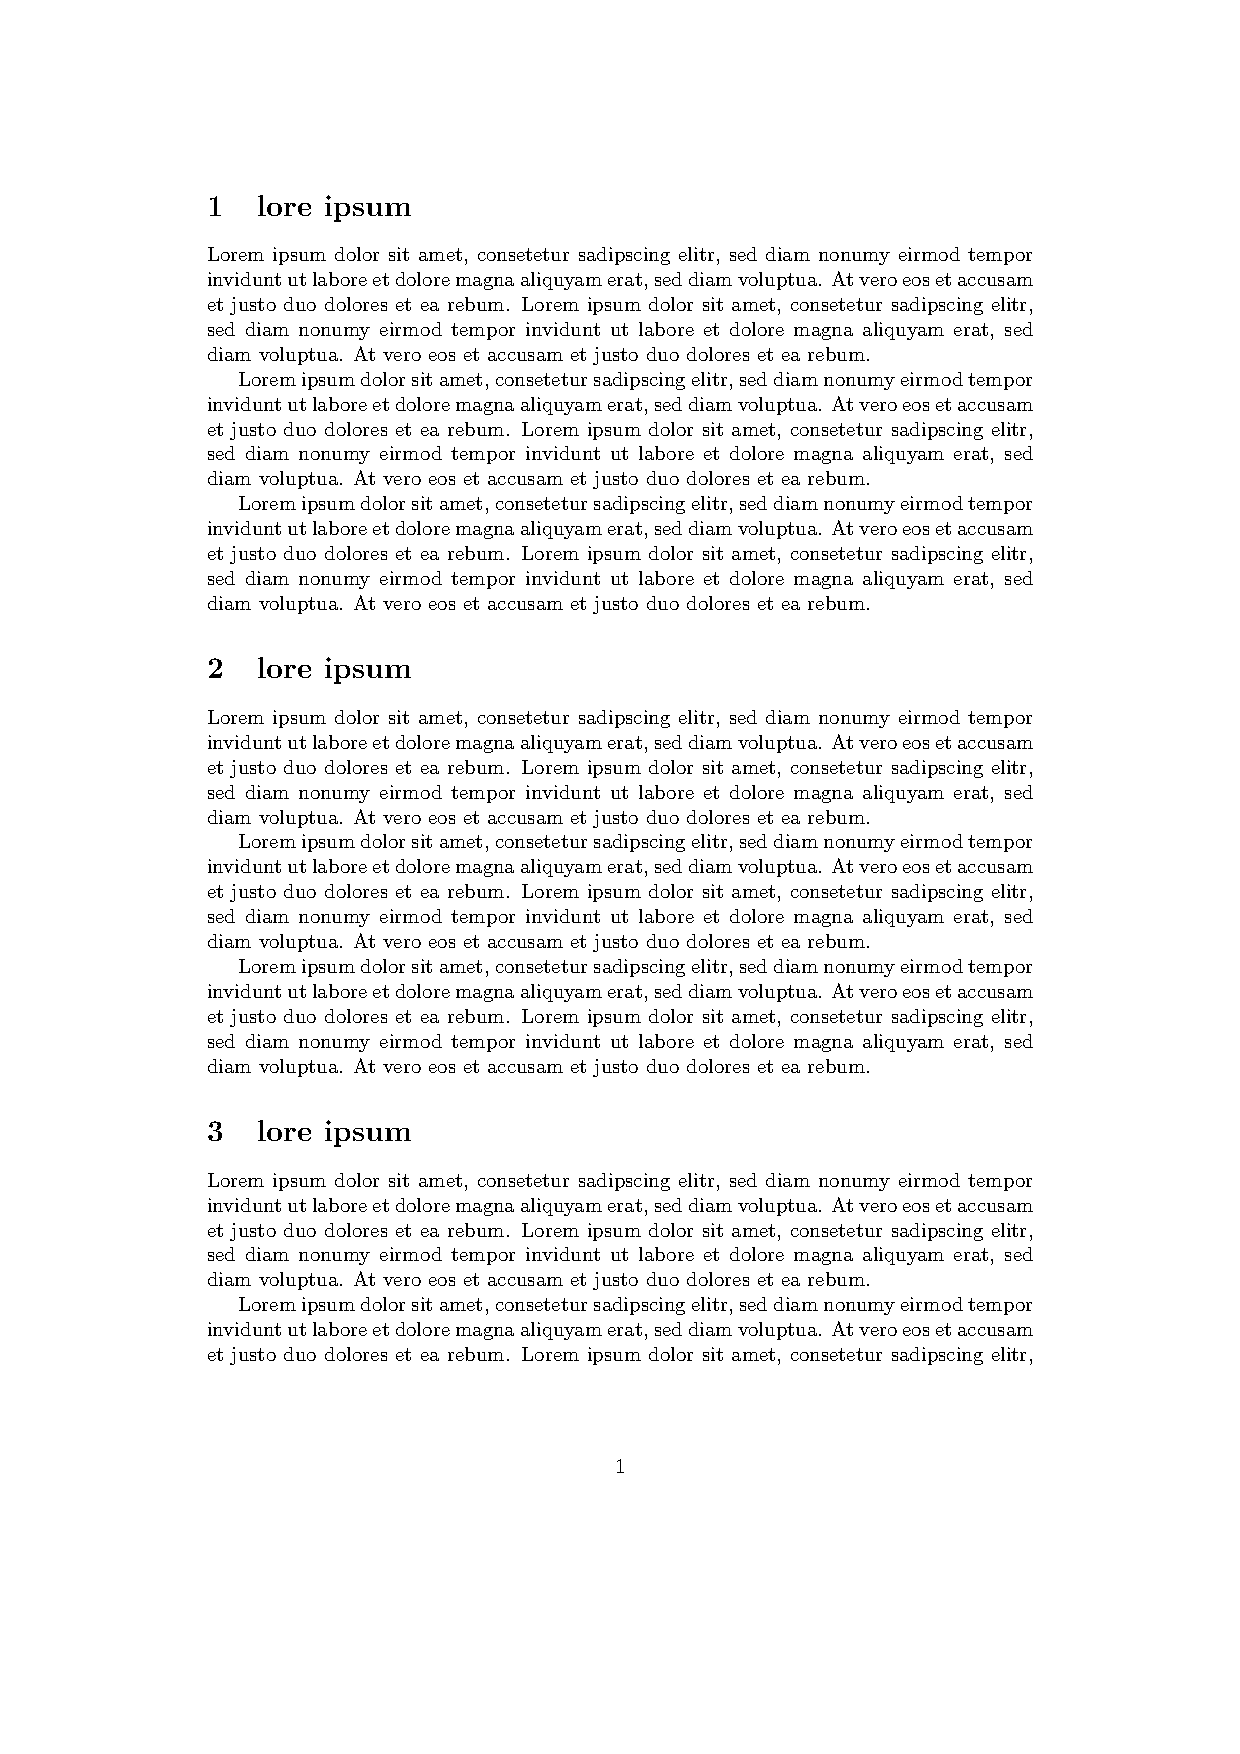
\includepdf[pagetemplate=7, pages=-, nup=3x3,
            frame]{pdf/mix1.pdf}

Protr"at-Dokument, das mit Landscape beginnt: zuerst falsch
\begin{verbatim}
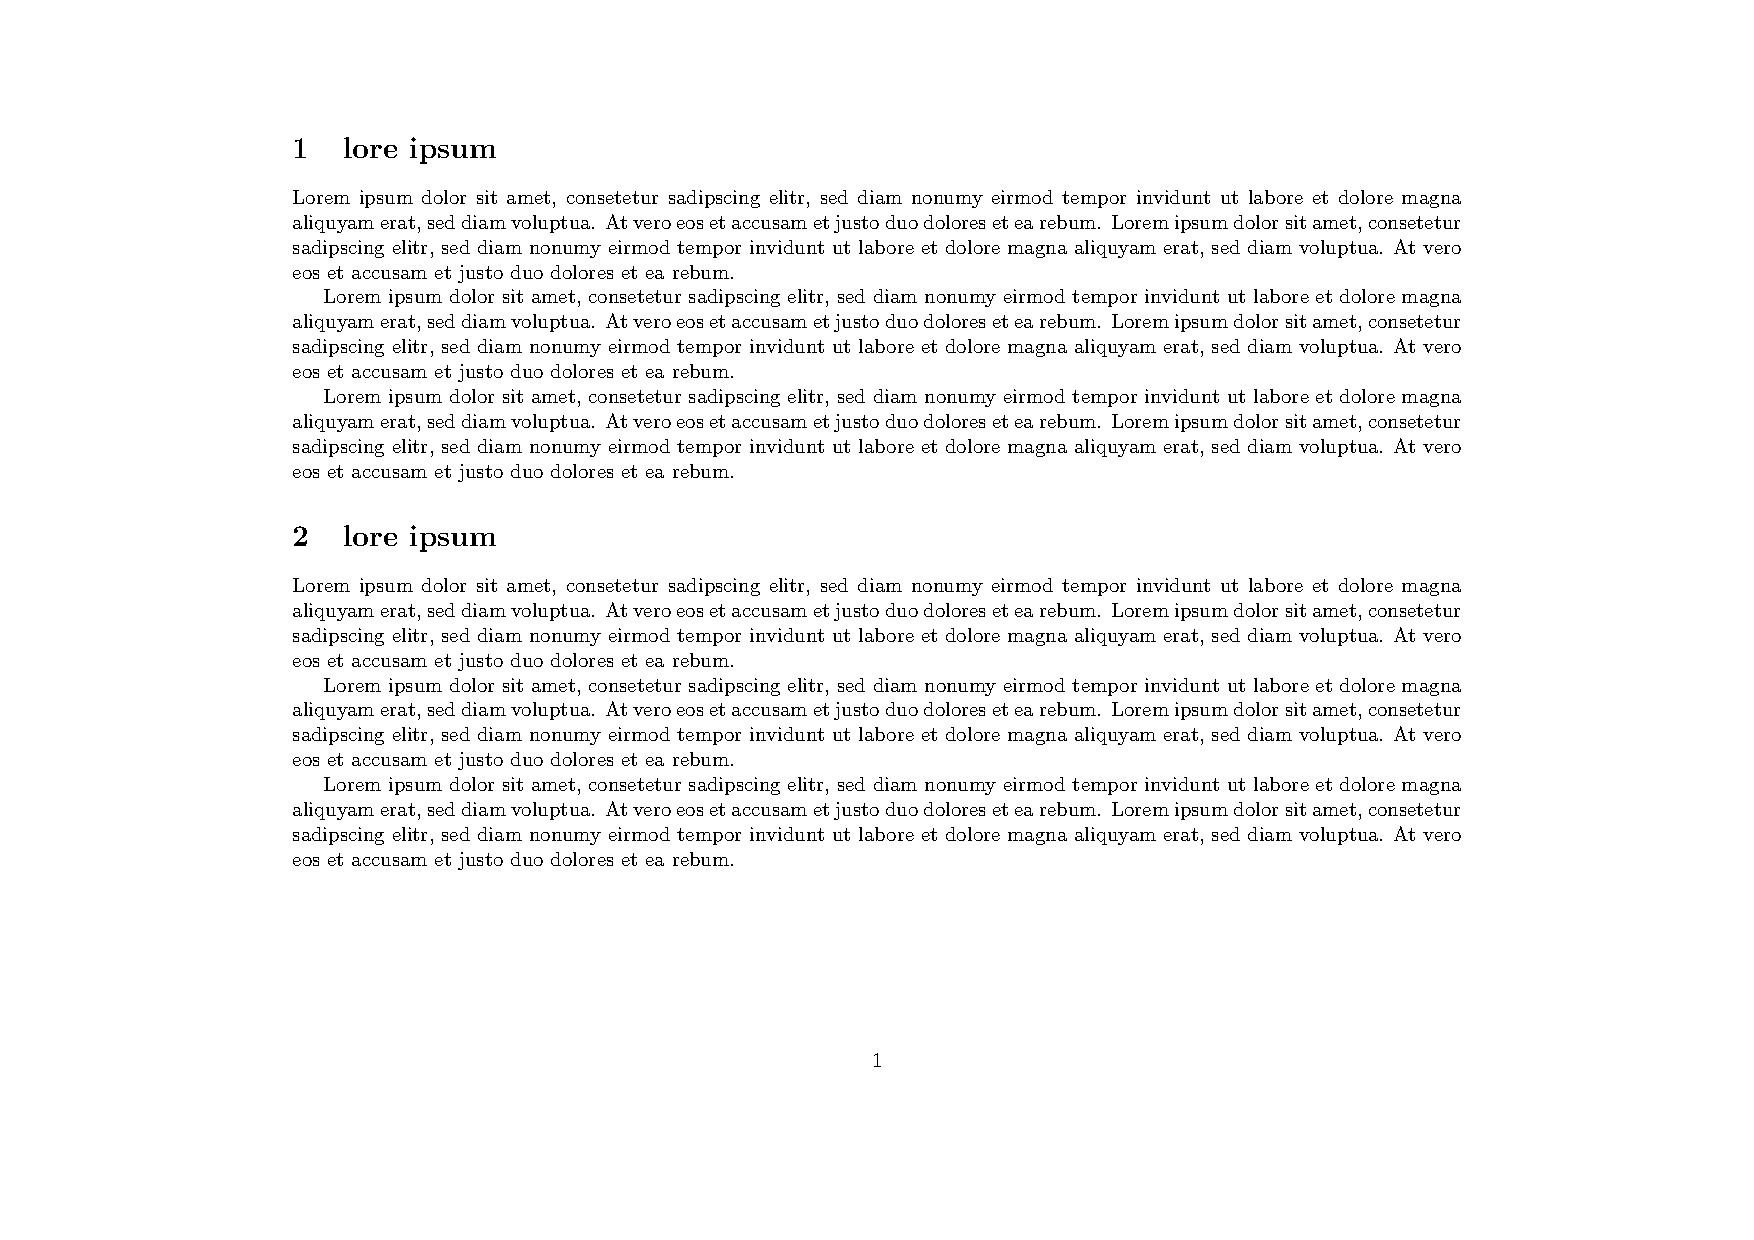
\includepdf[pages=-, nup=2x2, frame]{pdf/mix2.pdf}
\end{verbatim}
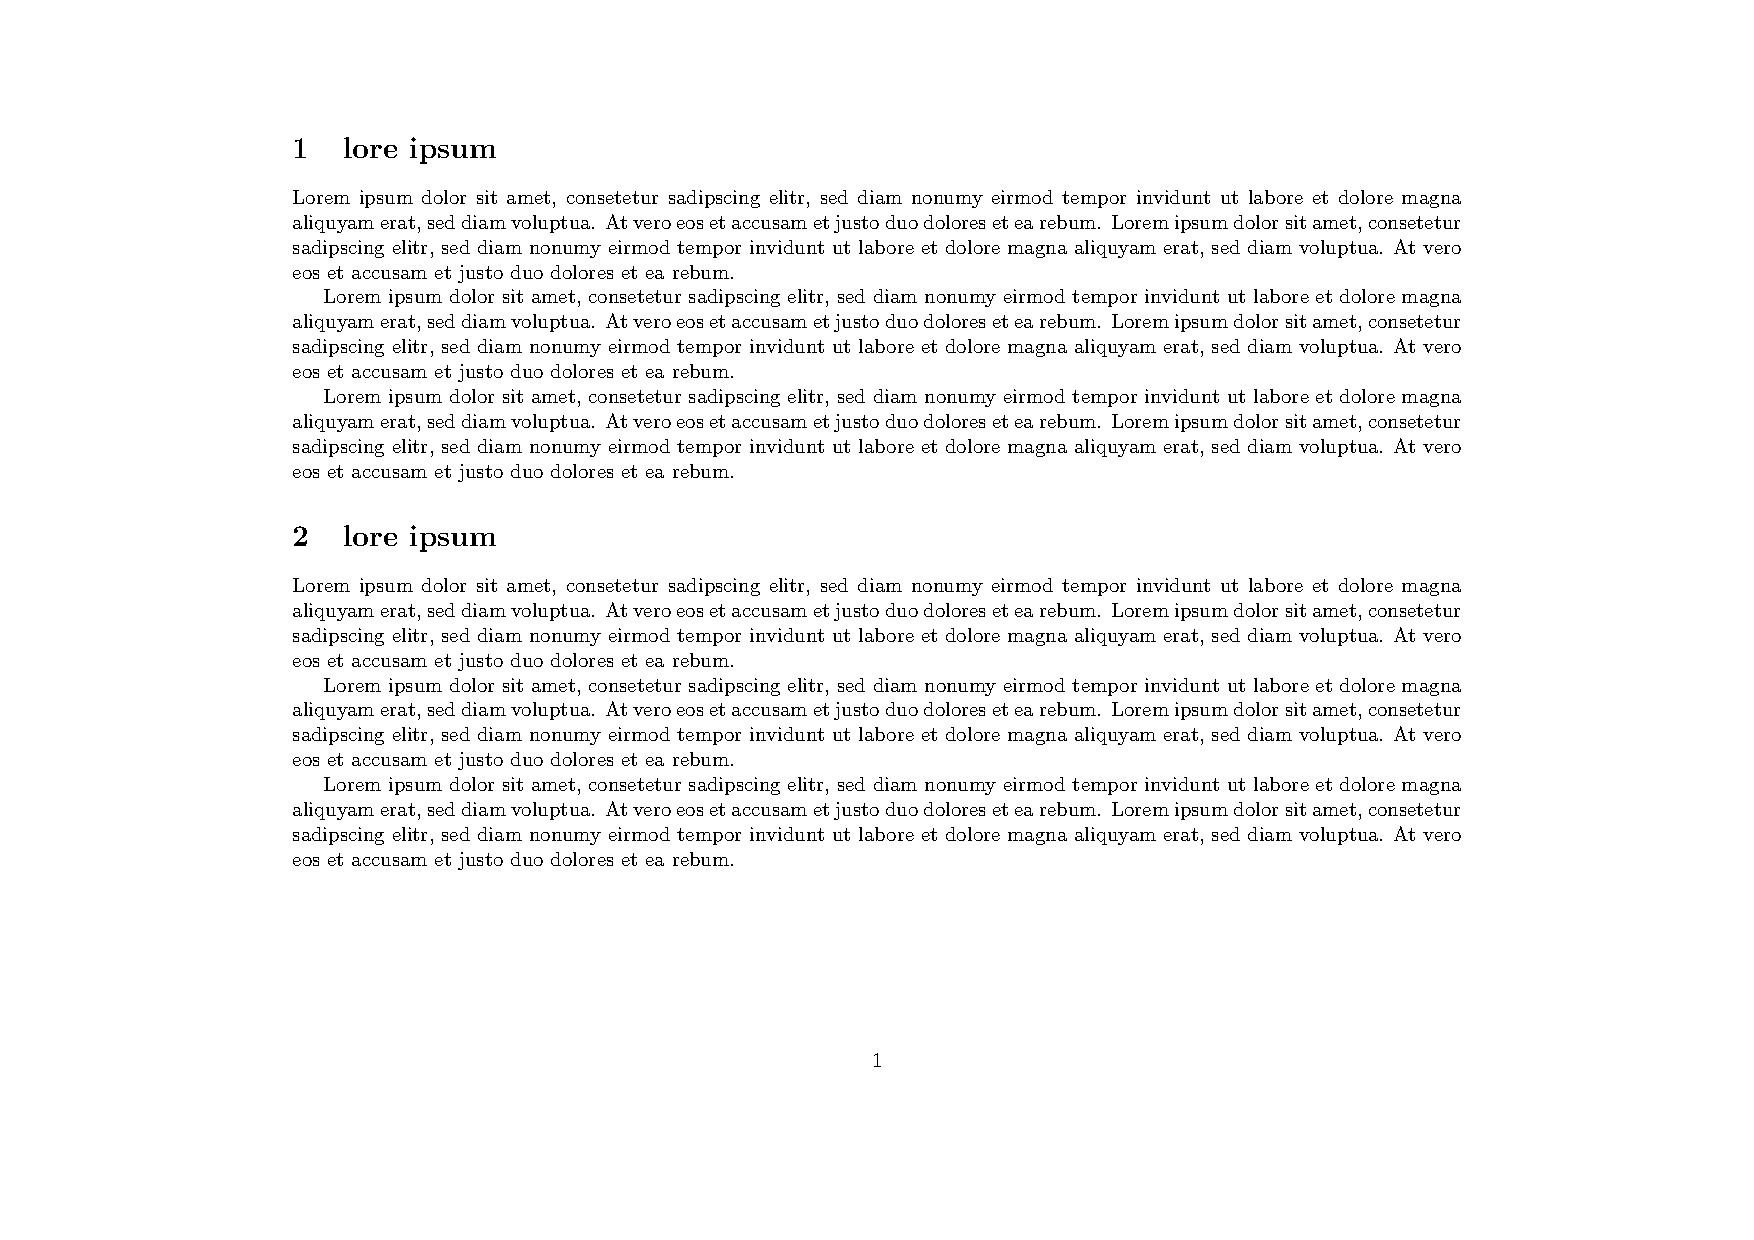
\includepdf[pages=-, nup=2x2, frame]{pdf/mix2.pdf}

jetzt richtig, ohne drehen
\begin{verbatim}
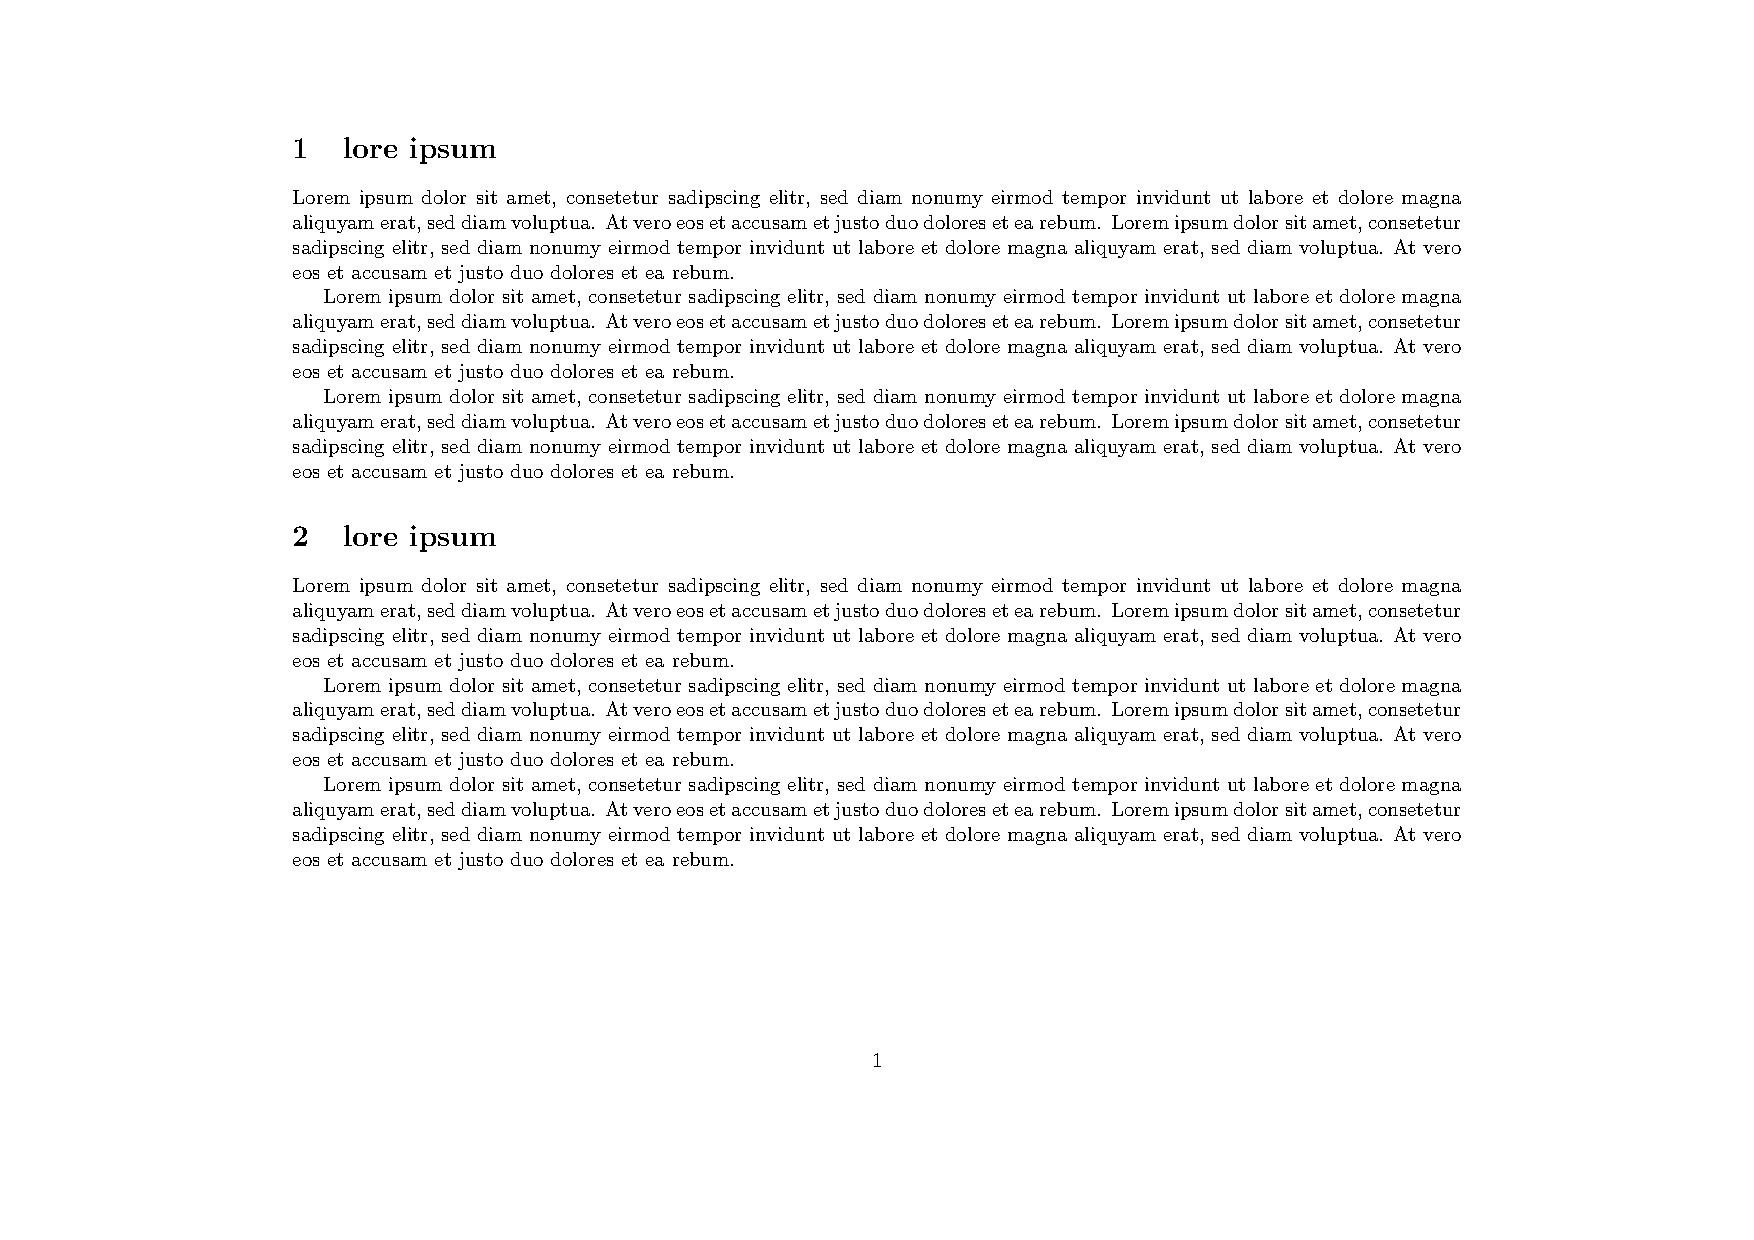
\includepdf[pagetemplate=2, pages=-, nup=2x2,
            frame]{pdf/mix2.pdf}
\end{verbatim}
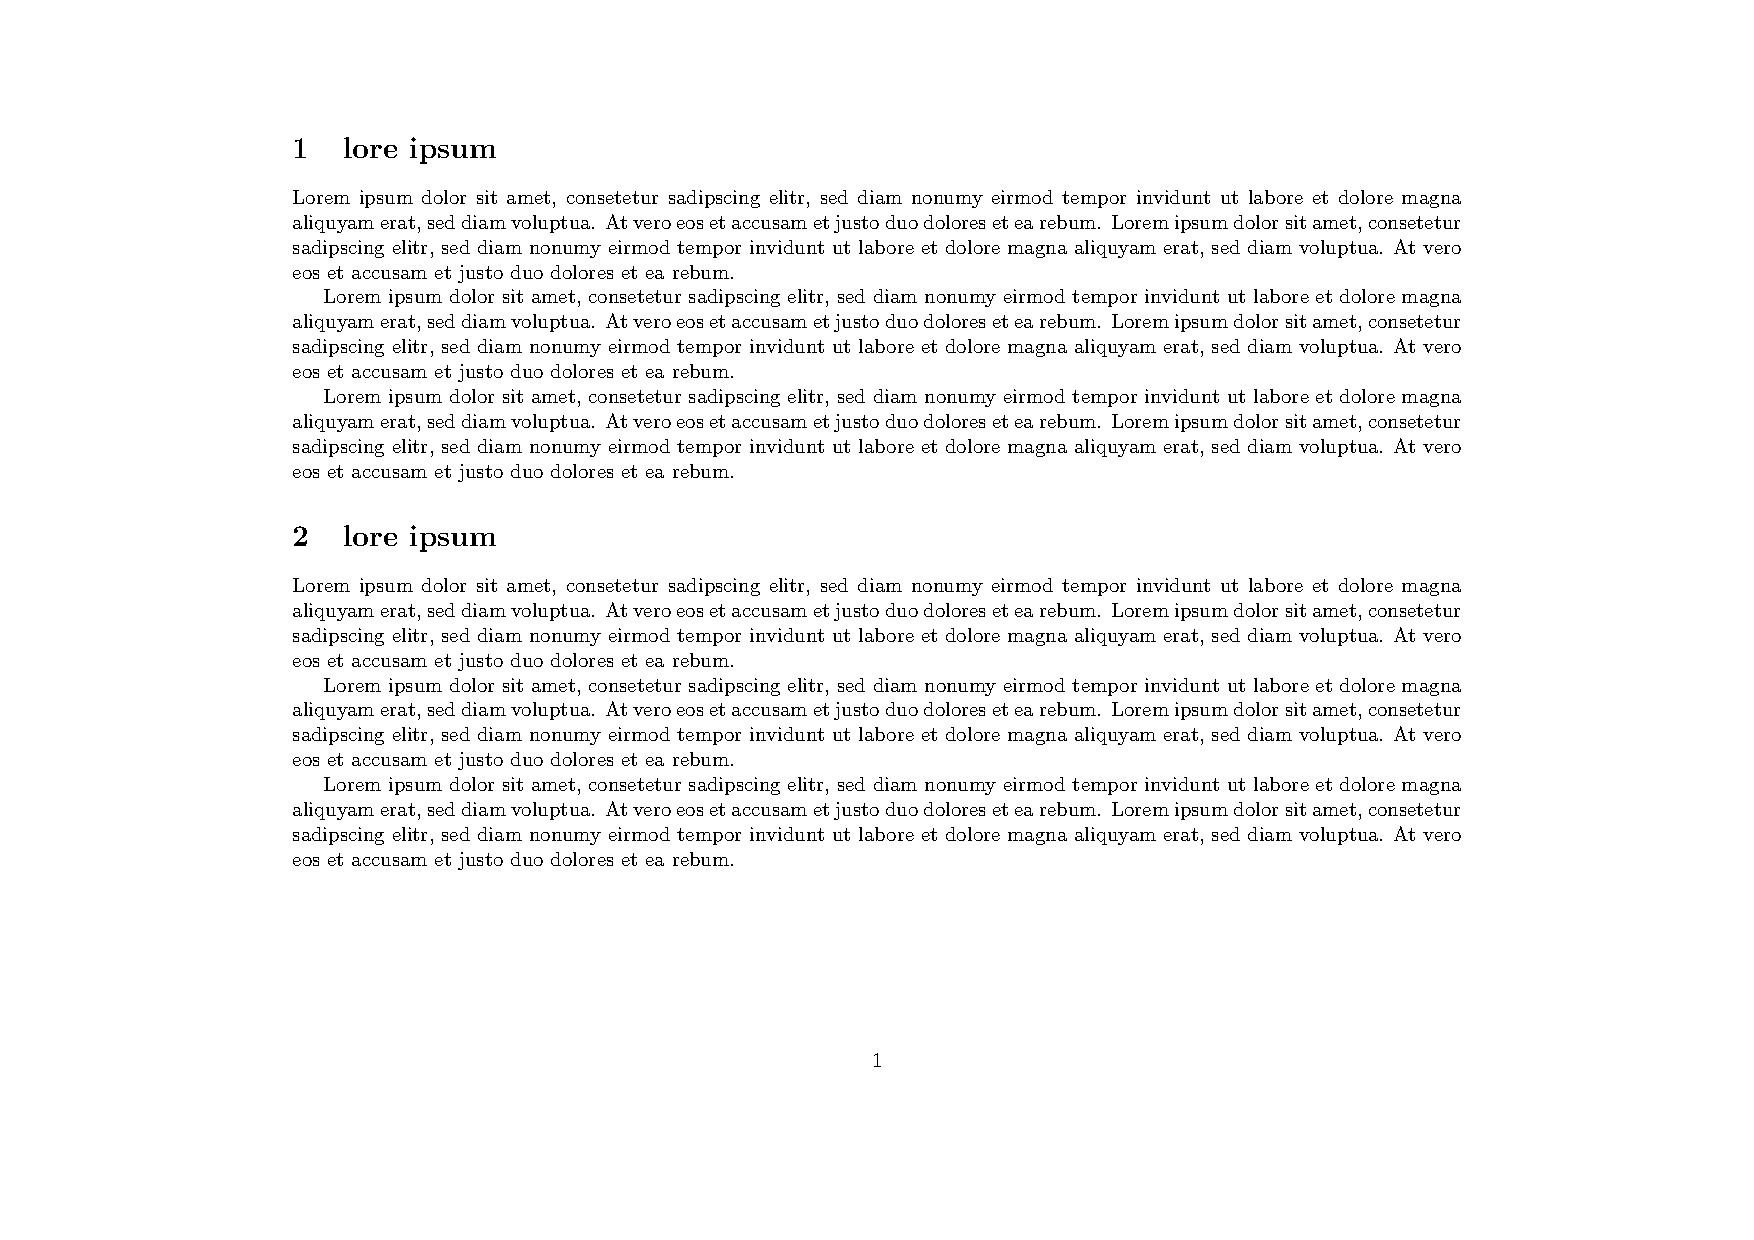
\includepdf[pagetemplate=2, pages=-, nup=2x2,
            frame]{pdf/mix2.pdf}

richtig, mit drehen
\begin{verbatim}
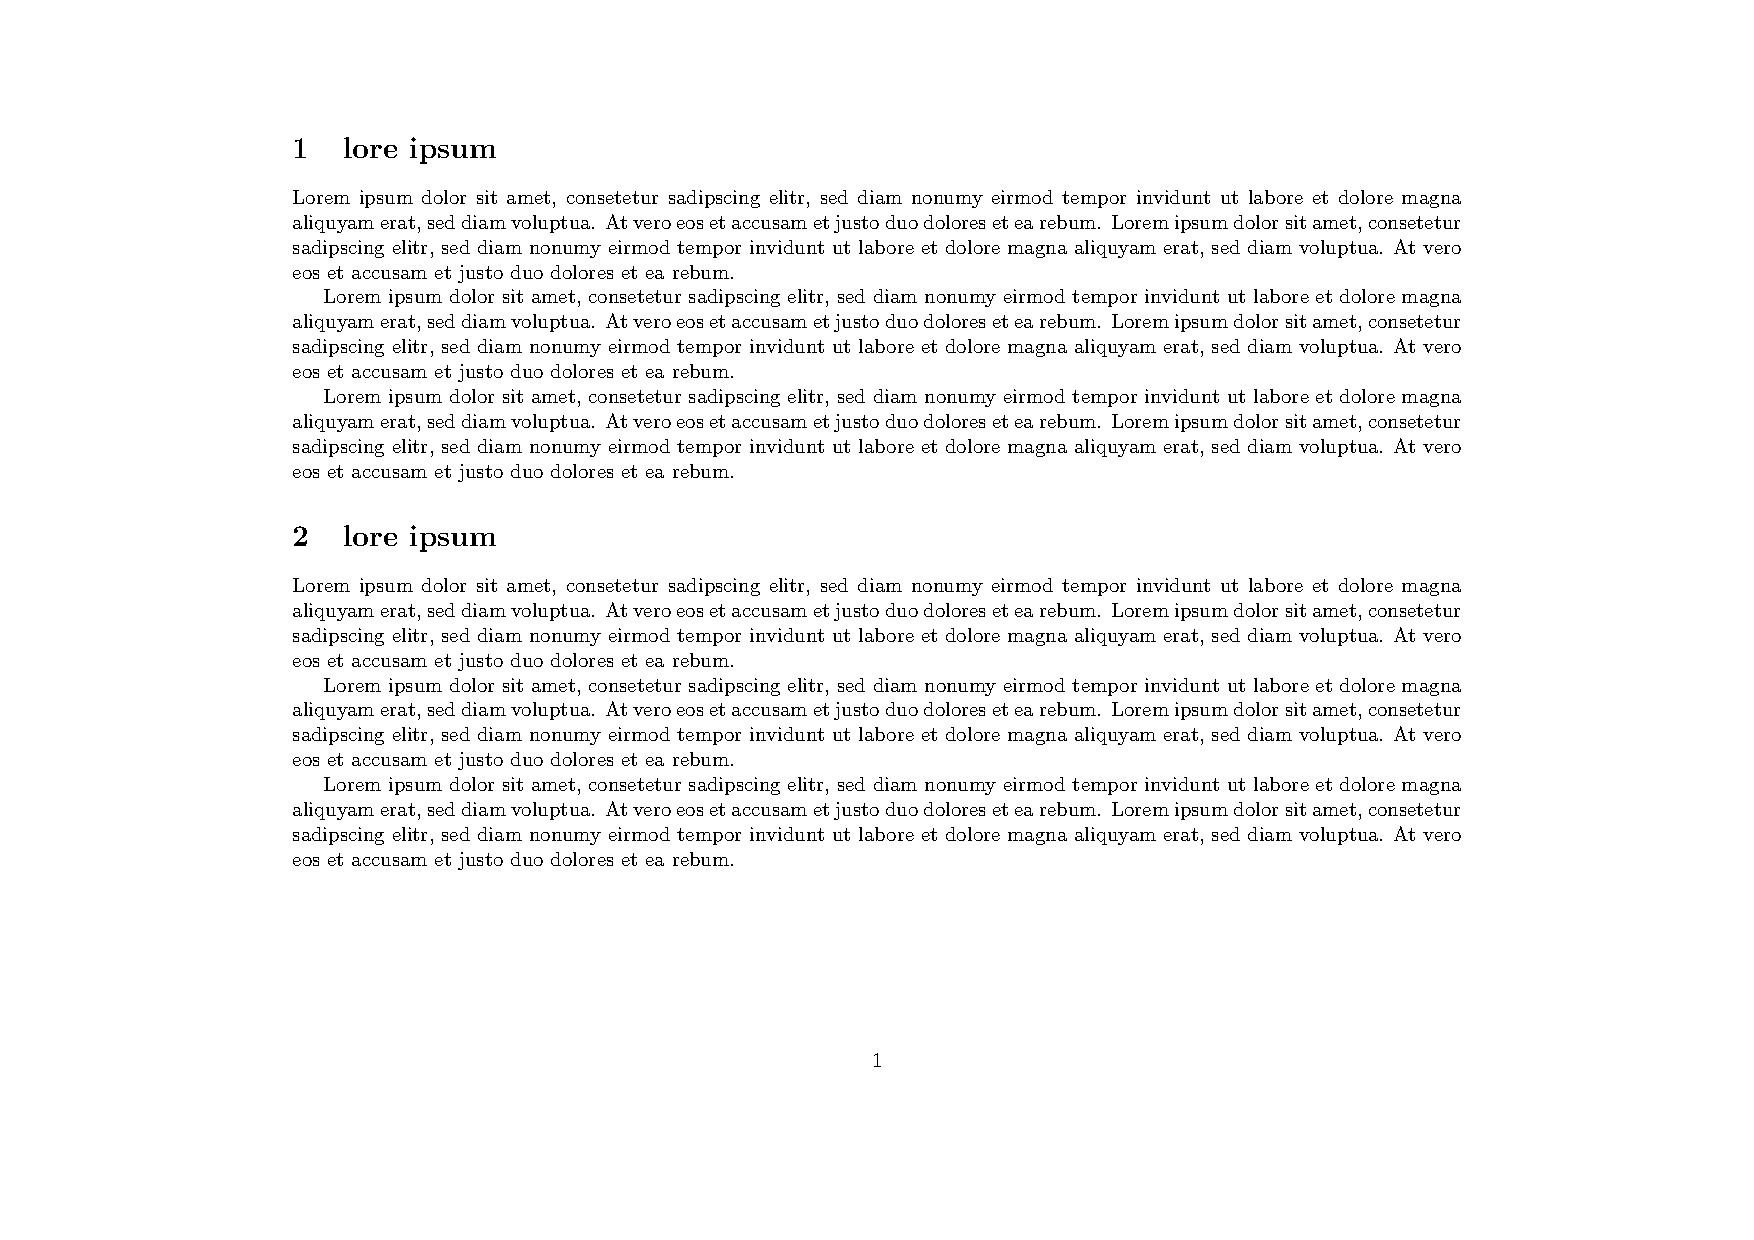
\includepdf[rotateoversize, pagetemplate=2,
            pages=-, nup=2x2, frame]{pdf/mix2.pdf}
\end{verbatim}
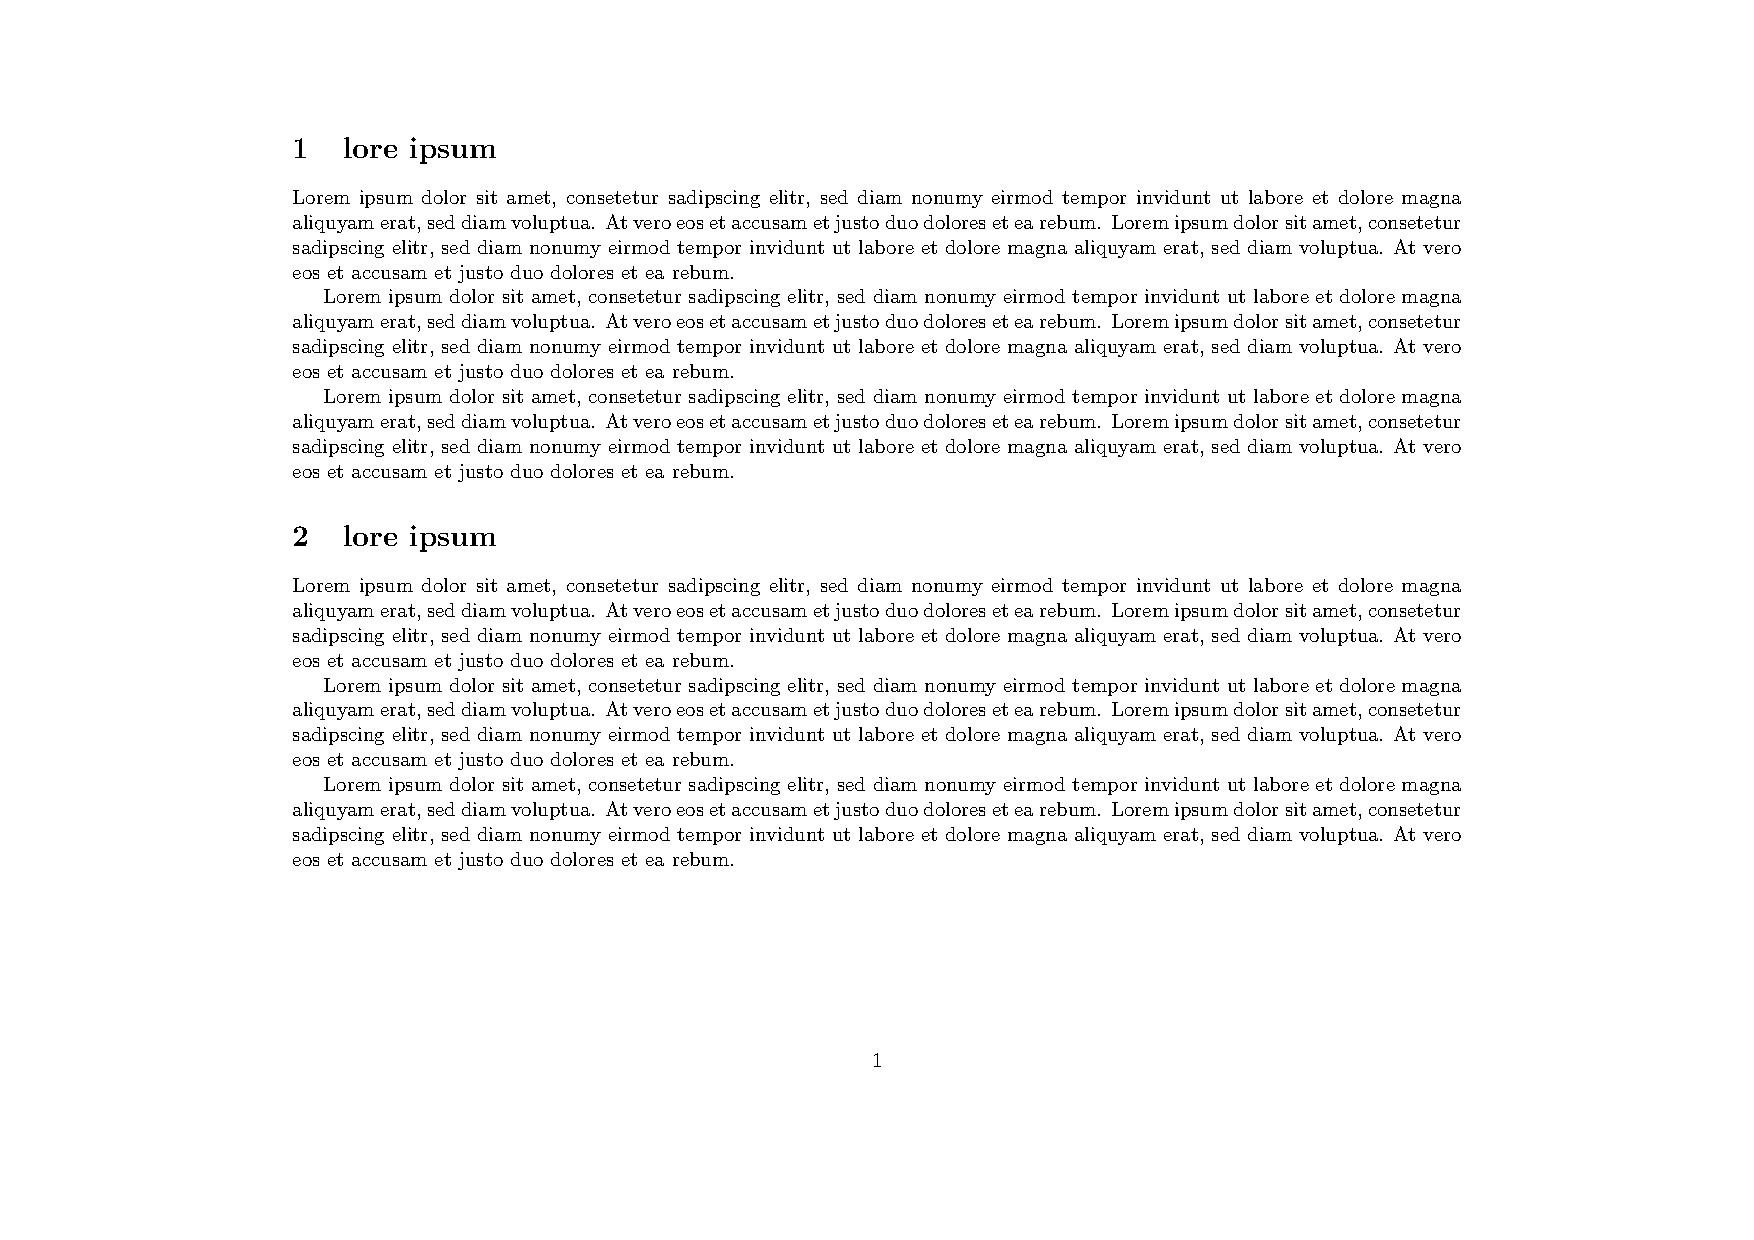
\includepdf[rotateoversize, pagetemplate=2,
            pages=-, nup=2x2, frame]{pdf/mix2.pdf}

\end{document}
